\section{A Running Example: DrawableDeck}~\label{sec:overview}
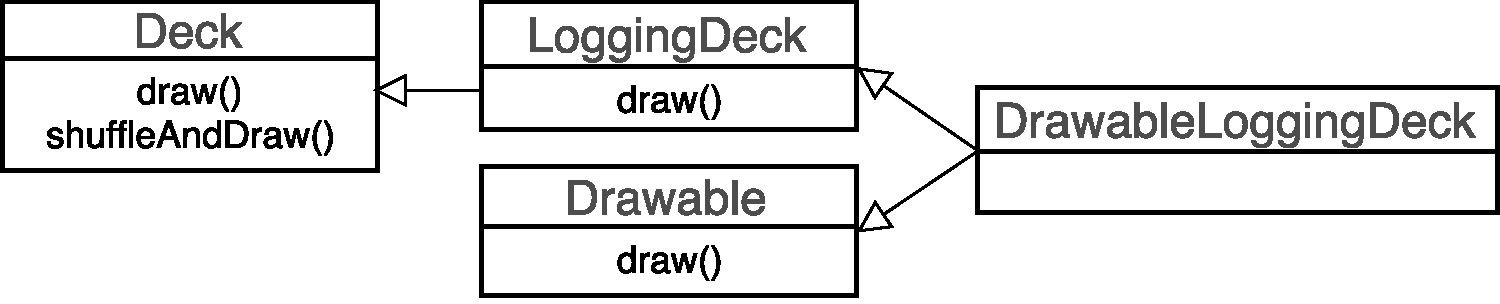
\includegraphics[height=3.3cm]{pics/DrawableLoggingDeck.pdf}
\red{H: with UML graphs the illustration could be better.}
This section illustrates the features of our \MIM{} model for resolving unintentional method
conflicts. As mentioned before, such a case arises when two inherited methods happen to have the
same signature, but with different semantics and functionalities. This could be quite troublesome
to programmers that use multiple inheritance. Below we illustrate with a running example called \lstinline|DrawableDeck|.
Note that we use Java-like syntax throughout the paper, and all types are defined with the keyword ``\lstinline|interface|'', which
supports multiple inheritance. Since \MIM{} is designed to be simple, we do not allow abstract methods, that is every method
is required to have a body for its implementation. In that case, interfaces can be directly instantiated by the keyword ``\lstinline|new|''
to create an object.

\subsection{Problem: Unintentional Method Conflicts}

Suppose that two components \lstinline|Drawable| and \lstinline|Deck| have been developed in a system.
\lstinline|Drawable| defines an interface for graphics that can be drawn, which includes a method called \lstinline|draw()|
for visual display. While interface \lstinline|Deck| represents a deck of cards, and supports several operations, like
\lstinline|draw()| for drawing a card from the deck.

\vspace{3pt}\begin{lstlisting}
interface Deck {
  void draw() { // draws a card from the Deck
    Stack<Card> cards = this.getStack();
    if (!cards.isEmpty()) {
      Card card = cards.pop();
      ...
    }
  }
}

interface Drawable {
  void draw() { // draws something on the screen
    JFrame frame = new JFrame("Canvas");
    frame.setVisible(true);
    ...
  }
}
\end{lstlisting}\vspace{3pt}
Note that both methods have \lstinline|void| return type (we will not formalize
\lstinline|void| in our calculus afterwards; here is only for illustration). In \lstinline|Deck|, \lstinline|draw()| tries to get the cards as a stack, pops
out the top card, and so on. While in \lstinline|Drawable|, \lstinline|draw()|
creates a blank canvas using \lstinline|JFrame|. Now, a programmer is designing a
card game with GUI. He may want to draw a deck on the screen, so he defines a drawable
deck using multiple inheritance:

\vspace{3pt}\begin{lstlisting}
interface DrawableDeck extends Drawable, Deck {
  ...
} 
\end{lstlisting}\vspace{3pt}
The point of using multiple inheritance is surely for composing the features of
components, achieving great code reuse. It is supported by many mainstream OO
languages. Nevertheless at this point, \lstinline|DrawableDeck| has to throw a compile
error, for the two \lstinline|draw()| methods cause a conflict, though accidentally.

\subsection{Potential Fixes}

For that problem, there are several workarounds that quickly come to our mind:

\paragraph{I. Delegation.} As an alternative to multiple inheritance, delegation can be used by
introducing two fields with \lstinline|Drawable| type and \lstinline|Deck| type, respectively. This avoids
method conflicts, nevertheless, delegation itself is too restricted in modularity, and meanwhile
introduces a lot of boilerplate.

\paragraph{II. Creating a \lstinline|draw()| method in \lstinline|DrawableDeck|, which explicitly overrides the old ones.}
This is a non-solution. It does not make any sense to override both methods with totally different functionalities, as old
methods have to be hidden.

\paragraph{III. Choosing one of them as the default method, like Mixins.} The mixin model can be applied to choose a
default one based on linearisation. Similarly, we want to preserve both features, rather than keeping only one of them.

\paragraph{IV. Method exclusion like traits.} Same reason as above.

\paragraph{V. Method renaming like traits.} This is probably what people do in most cases, by simply renaming one to avoid conflicts.
It can indeed preserve both features, however, it is cumbersome in practice, as introducing new names can affect other code blocks.
Certainly this is a workaround, not a solution.\\

What we really expect from the language is we keep both methods without renaming, and the type checker does not complain on the
inheritance. But we need to find an approach to disambiguate on method calls statically.

Certainly the compiler can ignore the conflict when \lstinline|DrawableDeck| is declared, but once an object of \lstinline|DrawableDeck| is created, a method call for \lstinline|draw()| on that object is ambiguous, due to dynamic dispatch. Nonetheless, we can adopt static dispatch for disambiguating. Some languages like C++ use qualified names in that way:

\vspace{3pt}\begin{lstlisting}
void func(Drawable obj) {
  obj.draw();
}

DrawableDeck d = new DrawableDeck();
d.Drawable::draw();       // calling draw() in Drawable
((Drawable) d).draw(); // calling draw() in Drawable
func(d);                 // calling draw() in Drawable
\end{lstlisting}\vspace{3pt}
Thus we have: \paragraph{VI. Static dispatch.} Static dispatch finds out and invokes the most specific method ``by need''.

On the other hand, we also need dynamic dispatch as it is essential and widely used in object-oriented programming.
C++ has the flexibility for choosing either way of dispatch by the ``virtual'' keyword.
Unfortunately, this approach is still unsatisfactory regarding code reuse. For instance, here we redefine \lstinline|Deck| to support
both \lstinline|draw()| and another operation called \lstinline|shuffleAndDraw()|:
\vspace{3pt}\begin{lstlisting}
interface Deck {
  void draw() {...}
  void shuffleAndDraw() {
    shuffle();
    draw();
  }
  ...
}
\end{lstlisting}\vspace{3pt}
\lstinline|shuffleAndDraw()| is a representative method that invokes \lstinline|draw()| in its definition. In principle, we want
that invocation to use dynamic dispatch, because a programmer may define a subtype of \lstinline|Deck|, and override \lstinline|draw()|:
\vspace{3pt}\begin{lstlisting}
interface LoggingDeck {
  void draw() { // overriding
    Stack<Card> cards = this.getStack();
    if (!cards.isEmpty()) {
      Card card = cards.pop();
      println("The card is: " + card.toString());
      ...
    } else {
      println("Empty deck.");
    }
  }
}
\end{lstlisting}\vspace{3pt}
Usually we want to reuse the code of \lstinline|shuffleAndDraw()| during inheritance, hence dynamic dispatch is necessary, otherwise
programmers have to override all the other methods that invoke \lstinline|draw()|. However, as seen before, dynamic dispatch can cause
ambiguity if we have:
\vspace{3pt}\begin{lstlisting}
interface DrawableLoggingDeck extends Drawable, LoggingDeck {
  ...
}

DrawableLoggingDeck d = new DrawableLoggingDeck();
d.shuffleAndDraw(); // ambiguous draw()
\end{lstlisting}\vspace{3pt}
Since the dynamic type of the receiver is \lstinline|DrawableLoggingDeck|, calling \lstinline|shuffleAndDraw()| triggers the ambiguity. When \lstinline|shuffleAndDraw()| invokes \lstinline|draw()|, what we really want is \lstinline|LoggingDeck.draw()|, yet
neither static dispatch nor dynamic dispatch in languages like C++ does so.
 Therefore, we need to find another algorithm for method binding.

\subsection{Solution in \MIM: \dispatchnamecaptical}
Our \MIM{} model uses \dispatchnameit{} for method lookup. A qualified method invocation, for instance, \lstinline|e.I::m()|, is read as ``finding the most specific \lstinline|m()| along path \lstinline|I|''. The meaning of ``along path \lstinline|I|'' is that, if the result of \dispatch{} is \lstinline|J.m()| for some \lstinline|J|, then such a \lstinline|J| must be a super type of \lstinline|e|'s dynamic type, and \lstinline|J| has a subtyping relation with \lstinline|I| (either \lstinline|J <: I| or \lstinline|J >: I|). Intuitively, the most specific \lstinline|m()| must be from branch \lstinline|I|, but it can be an overridden version after \lstinline|I| like dynamic dispatch. The formal definition will be introduced later.

On the other hand, \lstinline|((I) e).m()|, or simply \lstinline|e.m()| where \lstinline|e| has static type \lstinline|I|, behaves the same as \lstinline|e.I::m()| in our model. Such a dispatch make uses of both the static type and the dynamic type of the receiver. Intuitively, the static type specifies one branch of the method to avoid ambiguity, and the dynamic type finds the latest version on that branch. It may still introduce ambiguity when there are multiple paths from the static type to the dynamic type, and those paths cause conflicts. To prevent this, we disallow this kind of conflict to ensure unambiguity. That is to say, we do not allow two methods to override a same base method when they cause conflicts. This is natural, as they are just two versions of the same operation, hence it is no longer an ``unintentional'' conflict in that way.

With the old example, below code meets our expectation:
\vspace{3pt}\begin{lstlisting}
interface Deck {
  void draw() {...}
  void shuffleAndDraw() {
    this.Deck::shuffle();
    this.Deck::draw();
  }
  ...
}
\end{lstlisting}\vspace{3pt}
It guarantees that \lstinline|shuffleAndDraw()| are calling \lstinline|shuffle()| and \lstinline|draw()| from its own branch, so that the namesakes
from other branches will not cause conflicts. Now \lstinline|d.shuffleAndDraw()| is no longer ambiguous.

Actually in \MIM{}, we can still write ``\lstinline|shuffle();|'' and ``\lstinline|draw();|'',
because the compiler is able to know that the receiver ``\lstinline|this|'' exactly has static type \lstinline|Deck|, hence hierarchical dispatch eliminates ambiguity.

\subsection{Method Update in \MIM	}

\MIM{} supports two kinds of polymorphism on methods: (1) method overriding; (2) method update. A method update is similar to overriding, in the sense that it provides a refined implementation of a method. But the difference is that an update just refines one branch, since \MIM{} can preserve several conflicted branches at the same time. Whereas a method overriding will hide all its inherited original methods, in which case method conflicts are unexpectedly ignored.

For example, we define an interface \lstinline|DrawableLoggingDeck2|, where we refine the \lstinline|draw()| from \lstinline|Drawable()| by setting
the canvas invisible:
\vspace{3pt}\begin{lstlisting}
interface DrawableLoggingDeck2 extends DrawableLoggingDeck {
  void draw() updates Drawable {
    JFrame frame = new JFrame("Canvas");
    frame.setVisible(false);
    ...
  }
}
\end{lstlisting}\vspace{3pt}
Here the update specifies \lstinline|Drawable| to be refined. The use of this update ensures that both branches of \lstinline|draw()| are preserved. At the same time, we should notice that a method update is no longer considered as an original method. Some client code is shown below:
\vspace{3pt}\begin{lstlisting}
DrawableLoggingDeck2 d2 = new DrawableLoggingDeck2();
d2.Drawable::draw(); // calling draw() in DrawableLoggingDeck2
d2.Deck::draw();       // calling draw() in LoggingDeck
\end{lstlisting}\vspace{3pt}

In \MIM{}, hierarchical dispatch first finds the most specific original method (with respect to method overriding), then it finds the most specific update on that method. A counter-example is when there are two method updates on \lstinline|Drawable| in \lstinline|DrawableLoggingDeck2|, it leads to ambiguity. The compiler is supposed to forbid that during compile time.

Two rules for method updates in \MIM: updates can only refine \textbf{original} methods, and they cannot overlap method overriding. For instance, writing \lstinline|"void draw()| \lstinline|updates Deck {...}"| is disallowed in \lstinline|DrawableLoggingDeck2|, because existing two branches are \lstinline|Drawable.draw()| and \lstinline|LoggingDeck.draw()|, yet \lstinline|Deck.draw()| is already overridden. It does not really make sense to update the old branch.

Similar to many OO languages, \MIM{} also allows \textit{super method invocation} in a method body. The invocation \lstinline|super.T::m()| will ignore all the subtypes of \lstinline|T|, and only look at \lstinline|T| together with its super interfaces.